\documentclass[10pt]{article}
\usepackage{pgfplots}
\pgfplotsset{compat=1.15}
\usepackage{mathrsfs}
\usepackage{tikz}
\usepackage{tkz-euclide}
\usetikzlibrary{arrows}
\pagestyle{empty}
\begin{document}
\definecolor{qqqqff}{rgb}{0,0,1}
\definecolor{ffqqqq}{rgb}{1,0,0}
\definecolor{ududff}{rgb}{0.30196078431372547,0.30196078431372547,1}
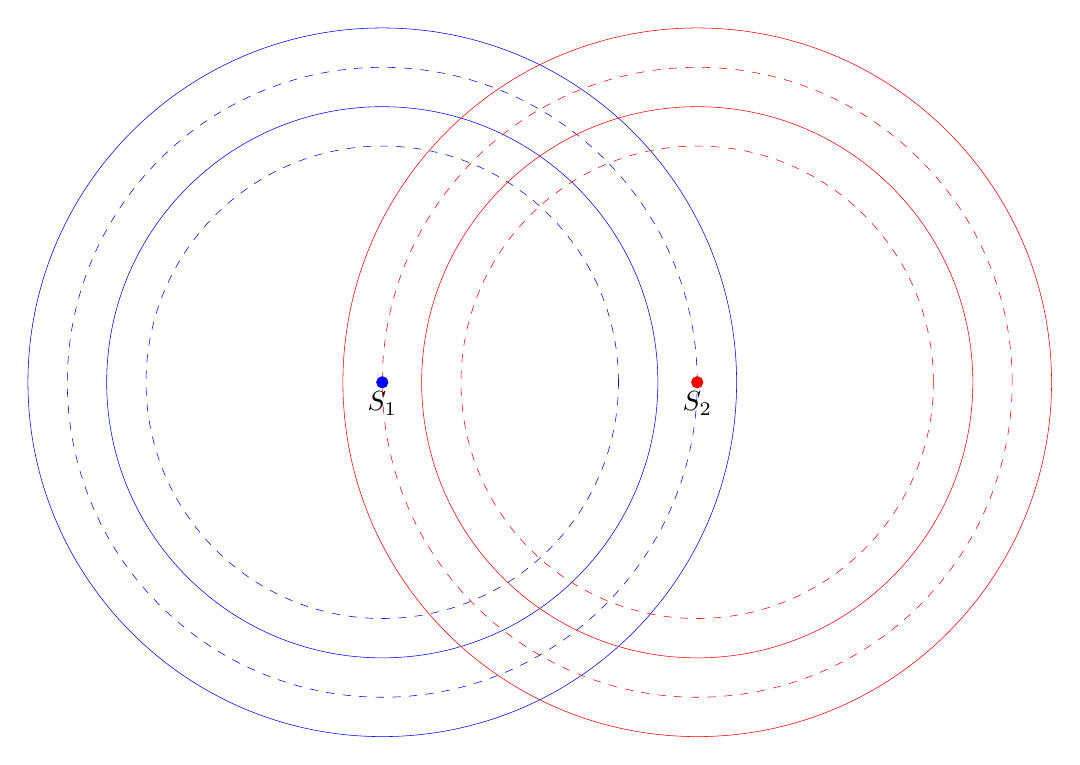
\begin{tikzpicture}[]
    \tkzDefPoints{-2/0/S1,2.5/0/S1_1UP,1.5/0/S1_2UP,2/0/S1_1DOWN,1/0/S1_2DOWN}
    \tkzDrawCircle[color=blue](S1,S1_1UP)
    \tkzDrawCircle[color=blue](S1,S1_2UP)
    \tkzDrawCircle[color=blue,style=dashed](S1,S1_1DOWN)
    \tkzDrawCircle[color=blue,style=dashed](S1,S1_2DOWN)
    
    \tkzDefPoints{2/0/S2,-2.5/0/S2_1UP,-1.5/0/S2_2UP,-2/0/S2_1DOWN,-1/0/S2_2DOWN}
    \tkzDrawCircle[color=red](S2,S2_1UP)
    \tkzDrawCircle[color=red](S2,S2_2UP)
    \tkzDrawCircle[color=red,style=dashed](S2,S2_1DOWN)
    \tkzDrawCircle[color=red,style=dashed](S2,S2_2DOWN)
    
    \tkzDrawPoint[color=blue,size=4pt](S1)
    \tkzDrawPoint[color=red,size=4pt](S2)
    \tkzLabelPoint(S1){\(S_1\)}
    \tkzLabelPoint(S2){\(S_2\)}
    
\end{tikzpicture}
\end{document}

